%!TEX root = forallxyyc.tex

\part{Lógica Modal}
\label{ch.ML}
\addtocontents{toc}{\protect\mbox{}\protect\hrulefill\par}

%\usepackage{gensymb}
%\input{fitch1.sty}

\chapter{Introduzindo a  lógica modal}
\label{Intro}

A lógica modal (LM) é a lógica que trata de modalidades, maneiras pelas quais uma afirmação pode ser verdadeira. As duas modalidades mais conhecidas são   \emph{Necessidade} e \emph{Possibilidade}. Uma afirmação pode ser verdadeira, mas também pode ser necessariamente verdadeira (verdadeira não importando como o mundo possa ser). Por exemplo, verdades lógicas não são apenas verdadeiras por causa de alguma característica acidental do mundo, mas verdadeiras em qualquer circunstância. Uma dada afirmação pode não ser realmente verdadeira, mas pode ter sido verdadeira. 
Usamos o operador modal $\ebox$ para expressar \emph{necessidade} e $\ediamond$ para expressar \emph{possibilidade}. Assim, você pode ler $\ebox \metav{A}$ como \emph{é necessariamente o caso que} $\metav{A}$, e $\ediamond \metav{A}$ como \emph{é possivelmente o caso que} $\metav{A}$.

Existem muitos tipos diferentes de necessidade e possibilidade. Por exemplo, é    \emph{humanamente impossível} correr a 200 km/h. Dado o tipo de criaturas que somos, nenhum ser humano pode fazer isso. Mas, ainda assim, não é \emph{fisicamente impossível} correr tão rápido. Ainda não temos a tecnologia para fazer isso, mas certamente é fisicamente possível trocar minhas pernas biológicas por pernas robóticas que possam funcionar a 200 km/h. Por outro lado, é fisicamente impossível correr a uma velocidade maior que a da luz, pois isso iria contra as leis da física. Entretanto, isso não é \emph{logicamente} impossível, pois não é uma contradição imaginar que as leis da física possam ser diferentes e que possam permitir que os objetos se movam mais rápido que a luz.

Com que tipos de modalidade a LM lida? \emph{Todos eles}! A LM é uma ferramenta muito flexível. Começamos com um conjunto básico de regras que regem os operadores modais $\ebox$ e $\ediamond$. Em seguida, adicionamos mais regras para adequar qualquer tipo de modalidade em que estamos interessados. Na verdade, a LM é tão flexível que nem precisamos pensar sempre em $\ebox$ e $\ediamond$ como expressando \emph{necessidade} e \emph{possibilidade} respectivamente. Em vez disso, podemos ler $\ebox$ como expressando \emph{demonstrabilidade}, de modo que $\ebox\metav{A}$ significa   \emph{é demonstrável que} $\metav{A}$, e $\ediamond\metav{A}$ significa \emph{não é refutável que} $\metav{A}$. Da mesma forma, podemos interpretar $\ebox\metav{A}$ como significando $S$ \emph{sabe que  $\metav{A}$} ou $S$ \emph{acredita que $\metav{A}$}. 
Ou ainda, podemos ler $\ebox$ como expressando \emph{obrigação moral}. Nesse caso, $\ebox \metav{A}$ significa \emph{é moralmente obrigatório que} $\metav{A}$ e $\ediamond \metav{A}$ significa \emph{é moralmente permissível que} $\metav{A}$. Tudo o que precisaríamos fazer é elaborar as regras corretas para essas diferentes leituras de $\ebox$ e $\ediamond$.

  Dependendo da interpretação que atribuímos aos operadores $\ebox$ e $\ediamond$, certas sentenças modais serão provadas ou válidas. Por exemplo, se $\ebox$ é interpretado como necessidade, a sentença `$\ebox A \eif A$' pode expressar `se $A$ é necessária, é verdadeira'.
  Sob essa  interpretação,  `$\ebox A \eif A$' é válida: todas as afirmações necessárias são verdadeiras aconteça o que acontecer, então são verdadeiras no mundo real. No entanto, quando   $\ebox$  é interpretado como “acredita-se que” ou “deveria ser o caso”,  a sentença 
  `$\ebox A \eif A$' não é válida: podemos acreditar em proposições falsas. Nem toda proposição que deveria ser verdadeira é de fato verdadeira como por exemplo, `Todo assassino será levado à justiça'. Isso \emph{deve}  ser verdadeiro, mas não o é.

Vamos apresentar diferentes tipos de sistemas da LM, a saber, os sistemas  \mlK, \mlT, \mlSfour{} e \mlSfive.  Eles diferem nas regras de derivação permitidas e na semântica que usaremos para definir nossas noções lógicas.  \mlK{} é o sistema  básico, pois tudo o que é válido ou provado em \mlK{} também pode ser provado nos outros sistemas. 
Veremos que a sentença  `$\ebox A \eif A$'   não é provada em \mlK, mas sim em  \mlT. Isto significa que o sistema \mlT{} é mais apropriado quando se trata de necessidade, porém menos apropriado quando se trata de crença ou obrigação.
 O  sistema  \mlSfive, por sua vez, além de ser considerado como o sistema que melhor captura os conceitos de possibilidade e necessidade lógica, é do ponto de vista dedutivo o sistema mais forte entre eles. 
 

\section{A linguagem da LM}
\label{TFLtoML}


A linguagem da LM é uma extensão da LVF. Tem um estoque infinito de \emph{letras sentenciais} (sentenças atômicas); os conectivos lógicos $\enot$, $\eand$,  $\eor$,    $\eif$  e $\eiff$; além dos  operadores modais  $\ebox$ e $\ediamond$.

Poderíamos ter começado com a LPO, o que nos teria dado a Lógica Modal Quantificada (LMQ). A LMQ é muito mais poderosa do que a LM, mas também é muito, muito mais complicada. Assim,  vamos manter as coisas simples e começar com uma extensão da LVF. 

As regras de construção de  sentenças da LM são todas da LVF mais duas novas regras para os operadores modais. Assim, temos a seguinte definição formal para uma sentença da LM:
 
\begin{itemize}
	\item[(1)]Toda letra sentencial é uma sentença. 
	\item[(2)]Se $\metav{A}$ é uma sentença, então $\enot\metav{A}$ é uma sentença. 
	\item[(3)]Se $\metav{A}$ e $\metav{B}$ são sentenças, então $(\metav{A}\eand\metav{B})$ é uma sentença.
	\item[(4)]Se $\metav{A}$ e $\metav{B}$ são sentenças, então $(\metav{A}\eor\metav{B})$ é uma sentença.
	\item[(5)]Se $\metav{A}$ e $\metav{B}$ são sentenças, então $(\metav{A}\eif\metav{B})$ é uma sentença.
	\item[(6)]Se $\metav{A}$ e $\metav{B}$ são sentenças, então $(\metav{A}\eiff\metav{B})$ é uma sentença.
	\item[(7)]Se $\metav{A}$ é uma sentença, então $\ebox\metav{A}$ é uma sentença.
	\item[(8)]Se $\metav{A}$ é uma sentença, então $\ediamond\metav{A}$ é uma sentença.
	\item[(9)]Nada além do estabelecido por essas cláusulas é uma sentença. 
\end{itemize}
Aqui estão alguns exemplos de sentenças  da LM:
\begin{itemize}
	\item[]$A,\;P\eor Q,\;\ebox A,\;C\eor \ebox D,\;\ebox\ebox (A\eif R)$ e 
	\item[]$\ebox\ediamond (S\eand (Z\eiff (\ebox W \eor \ediamond Q)))$
\end{itemize}

\chapter{Dedução natural para a LM}
\label{Proof}

Na Parte~\ref{ch.NDTFL},  apresentamos um sistema em dedução natural para a LVF, no qual, explicitamos as regras de inferência que regem os conetivos lógicos da  LVF.  Agora, sabendo que a linguagem da LM é uma extensão da LVF,  que além dos conectivos lógicos tem os operadores modais   $\ebox$ e $\ediamond$,  precisamos especificar as regras de inferência para tais operadores modais. Ora, é exatamente isso o que faremos neste capítulo. Vamos apresentar os sistemas em dedução  natural  para as lógicas modais  \mlK, \mlT, \mlSfour{} e \mlSfive.

Como  antes,  usaremos `$\proves$' para expressar dedutibilidade. Entretanto, será útil adicionar um subscrito para indicar em qual sistema modal estamos trabalhando. Assim, por exemplo, se quisermos dizer que podemos provar $\metav{C}$ a partir de $\metav{A}_1,\metav{A}_2, \dots \metav{A}_n$ \emph{no sistema}~\mlK, escrevemos: $\metav{A}_1,\metav{A}_2, \dots \metav{A}_n \proves_\mlK \metav{C}$.

\section{Sistema \mlK}
\label{K}

Começamos com um sistema modal particularmente simples, chamado \mlK{} em homenagem ao filósofo e lógico Saul Kripke. O sistema \mlK{} tem todas as regras de dedução natural da  LVF, incluindo as regras  básicas e as derivadas, além de  duas novas regras básicas para o operador modal \ebox{} e um tipo especial de subprova.   

Esse  tipo especial de subprova, que chamamremos de  \emph{subprova estrita}, parece uma subprova comum, exceto que tem um~\ebox{} em sua linha de suposição em vez de uma fórmula. Ela nos permite provar coisas e raciocinar sobre possibilidades alternativas. 
 
 O que podemos provar dentro de uma subprova estrita vale para qualquer possibilidade alternativa, em particular, em possibilidades alternativas onde as suposições em vigor em nossa prova podem não valer. Em uma subprova estrita, todas as suposições são desconsideradas, e não estamos autorizados a apelar para quaisquer linhas fora da subprova estrita (exceto conforme permitido pelas regras modais fornecidas abaixo).

A regra \ebox I nos permite derivar uma fórmula $\ebox \metav{A}$ se pudermos derivar $\metav{A}$ dentro de uma subprova estrita. Esse é  nosso método fundamental para introduzir \ebox{} nas provas. A ideia básica é bastante simples: se $\metav{A}$ é um teorema, então  $\ebox \metav{A}$ deve ser um teorema também (lembre-se de que chamar $\metav{A}$ de teorema é dizer que podemos provar $\metav{A}$ sem confiar em quaisquer suposições não descartadas).

Suponha que queremos provar `$\ebox(A\eif A)$'. A primeira coisa que precisamos fazer é provar que `$A\eif A$' é um teorema. Isso você já sabe como fazer na LVF,  simplesmente apresentando uma prova de `$A\eif A$'  como esta:
\[
	\begin{nd}
		\open
		\hypo{1}{A}
		\have{2}{A}\by{R}{1}
		\close
		\have{3}{A\eif A}\ci{1-2}
	\end{nd}
\]
Claramente, a prova de `$A \eif A$' não faz uso de nenhuma suposição não descartada.  Assim, para aplicar a regra \ebox I, precisamos apenas inserir essa prova dentro de uma subprova estrita, como segue:


\[\begin{nd}
		\open
		\hypo{1}{\ebox}
		\open
		\hypo{2}{A}
		\have{3}{A}\by{R}{2}
		\close
		\have{4}{A\eif A}\ci{2-3}
		\close
		\have{5}{\ebox(A\eif A)}\boxi{1-4}
\end{nd}\]

Apresentamos agora  a regra \ebox I, a regra de introdução para o operador modal \ebox .

\factoidbox{
	\[\begin{nd}
			\open
			\hypo[m]{m}{\ebox}
			\have[n]{n}{\metav{A}}
			\close
			\have[\,]{o}{\ebox\metav{A}}\boxi{m-n}
		\end{nd}\]
	Nenhuma linha acima da linha $m$ pode ser citada por qualquer regra dentro da subprova estrita iniciada na linha $m$, a menos que a regra explicitamente o permita.
}

É essencial enfatizar que na subprova estrita você não pode usar qualquer regra que apele a qualquer coisa que você provou fora da subprova estrita.  Veremos que existem exceções como por exemplo a regra \ebox E. Mas, essas regras determinam  explicitamente que podem ser usadas dentro de subprovas estritas e cita linhas fora da subprova estrita. Essa restrição é essencial, caso contrário, obteríamos resultados terríveis. Por exemplo, poderíamos fornecer a seguinte prova para justificar  $A\therefore \ebox A$:
\[\begin{nd}
		\hypo{1}{A}
		\open
		\hypo{2}{\ebox}
		\have{3}{A}\by{uso incorreto de R}{1}
		\close
		\have{4}{\ebox A}\boxi{2-3}
	\end{nd}
\]
Essa não é uma prova legítima, porque na linha 3 apelamos para a linha 1, usando a regra de reiteração. Mas a linha 1 vem antes do início da subprova estrita na linha 2, contrariando assim a restrição da regra \ebox I.

Dissemos acima que uma subprova estrita nos permite raciocinar sobre possíveis situações alternativas arbitrárias. O que pode ser provado em uma subprova estrita vale em todas as situações alternativas possíveis e, portanto, é necessário. Essa é a ideia por trás da regra \ebox I. Por outro lado, se assumimos que algo é necessário, assumimos que isso é verdadeiro em todas as situações alternativas possíveis. Assim, temos a regra \ebox E:


\factoidbox{
	\[\begin{nd}
			\have[m]{m}{\ebox\metav{A}}
			\open
			\hypo[\ ]{o}{\ebox}
			\have[n]{n}{\metav{A}}\boxe{m}
			\close
		\end{nd}\]
		 \ebox E só pode ser aplicada se a linha $m$ (contendo $\ebox A$) estiver \emph{fora} da subprova estrita na qual a linha $n$ cai, e essa subprova estrita não é ela própria parte de uma subprova estrita que não contém~$m$. 
		}

A regra \ebox E permite que você introduza $\metav{A}$ dentro de uma subprova estrita se você tiver $\ebox \metav{A}$ fora dessa subprova estrita. A restrição impõe que você só pode fazer isso na primeira subprova estrita,  não permitindo aplicar a regra \ebox E dentro de uma subprova estrita aninhada. Vejamos um exemplo de  uso incorreto de \ebox E.

\[\begin{nd}
	\have{1}{\ebox\metav{A}}
	\open
	\hypo{2}{\ebox}
	\open
	\hypo{3}{\ebox}
	\have{4}{\metav{A}}\by{uso incorreto de \ebox E}{1}
\close\close
\end{nd}\]
O uso incorreto da regra \ebox E  na linha~$4$ viola a condição, porque embora a linha~$1$ esteja fora da subprova estrita que termina na  linha~$4$, a subprova estrita contendo a linha~$4$ está dentro da subprova estrita começando na linha~$2$, que não contém a linha~$1$.

 
Vejamos agora um exemplo com aplicações corretas das regras \ebox I e \ebox E. 
\[
	\begin{nd}
		\hypo{1}{\ebox A}
		\hypo{2}{\ebox B}
		\open
		\hypo{3}{\ebox}
		\have{4}{A}\boxe{1}
		\have{5}{B}\boxe{2}
		\have{6}{A \eand B}\ai{4,5}
		\close
		\have{6}{\ebox(A \land B)}\boxi{3-6}
	\end{nd}
\]


Também podemos misturar subprovas regulares e subprovas estritas, como podemos ver na seguinte prova de  $\ebox (A \eif B) \proves_\mlK  \ebox A \eif \ebox B$.


\[\begin{nd}
		\hypo{1}{\ebox (A \eif B)}
		\open
		\hypo{2}{\ebox A}
		\open
		\hypo{3}{\ebox}
		\have{4}{A}\boxe{m}
		\have{5}{A \eif B}\boxe{1}
		\have{6}{B}\ce{4,5}
		\close
		\have{7}{\ebox B}
		\close
		\have{8}{\ebox A \eif \ebox B} \ci{2-7}
	\end{nd}\]
Essa é chamada  de \emph{regra de distribuição}, porque nos diz que $\ebox$ `distribui' sobre $\eif$.

As regras \ebox I e \ebox E parecem bastante simples e, de fato, \mlK{} é um sistema muito simples! Mas \mlK{} é mais poderoso do que você pode imaginar. Você também pode  provar outras coisas nele.

\section{Possibilidade}
\label{possibility}

Na seção anterior, vimos todas as regras básicas para \mlK. Mas você deve ter notado que todas essas regras eram sobre necessidade,  $\ebox$, e nenhuma delas era sobre possibilidade, $\ediamond$. Isso não é um problema uma vez que podemos \emph{definir} possibilidade em termos de necessidade:
\factoidbox{
$\ediamond\metav{A}=_{df} \enot \ebox\enot \metav{A}$
}
Em outras palavras, dizer que $\metav{A}$ é \emph{possivelmente verdadeira}, é dizer que $\metav{A}$   \emph{não é necessariamente falsa}. Como resultado, não é realmente essencial adicionar um símbolo novo para possibilidade  no sistema \mlK. Ainda assim, o sistema será \emph{muito mais} fácil de usar se o fizermos. Por isso, adicionaremos as seguintes regras de definição:
\factoidbox{
	\[\begin{nd}
			\have[m]{m}{\enot\ebox\enot \metav{A}}
			\have[\, ]{n}{\ediamond \metav{A}}\diadf{m}
		\end{nd}
	\]
	\[\begin{nd}
			\have[m]{m}{\ediamond \metav{A}}
			\have[\, ]{n}{\enot\ebox\enot \metav{A}}\diadf{m}
		\end{nd}\]
}
É importante ressaltar que essas regras registram apenas a maneira como  o operador $\ediamond$  é definido em termos de $\ebox$ e, do ponto de vista dedutivo, elas não representam nenhuma adição real ao sistema \mlK. Entretanto, além dessas,  será útil adicionar outras \emph{regras de conversão modal} que nos fornecem maneiras  diferentes de alternar  $\ebox$  e $\ediamond$:
 

\factoidbox{
	\[\begin{nd}
			\have[m]{m}{\enot\ebox \metav{A}}
			\have[\, ]{n}{\ediamond \enot\metav{A}}\mc{m}
		\end{nd}
	\]
	\[\begin{nd}
			\have[m]{m}{\ediamond \enot \metav{A}}
			\have[\, ]{n}{\enot\ebox \metav{A}}\mc{m}
		\end{nd}\]
	\[\begin{nd}
			\have[m]{m}{\enot\ediamond \metav{A}}
			\have[\, ]{n}{\ebox \enot\metav{A}}\mc{m}
		\end{nd}\]
	\[\begin{nd}
			\have[m]{m}{\ebox\enot \metav{A}}
			\have[\, ]{n}{\enot\ediamond\metav{A}}\mc{m}
		\end{nd}\]
}
Todas essas regras de conversão modal podem ser derivadas das regras básicas de \mlK, usando a  definição de $\ediamond$. 

No sistema   \mlK, escolhemos $\ebox$ como nosso símbolo modal primitivo e, em seguida, definimos $\ediamond$ em termos dele. Mas, poderíamos ter começado com $\ediamond$ como símbolo  primitivo, e então definido $\ebox$ como segue: $\ebox\metav{A} =_{df} \enot \ediamond \enot \metav{A}$. 
Assim,  não há nenhum sentido em que a necessidade seja de alguma forma mais \emph{fundamental} do que a possibilidade. A necessidade é tão fundamental quanto a possibilidade em contextos modais.

\section{Sistema \mlT}
\label{T}

O sistema  \mlK{}   é um sistema modal muito simples e  tão fraco que nem mesmo permite que você prove $\metav{A}$  a partir de $\ebox\metav{A}$.  Mas se estivermos pensando em $\ebox$ como expressando \emph{necessidade}, deveríamos ser capazes de fazer esta inferência: se $\metav{A}$ é \emph{necessariamente verdadeira}, então ela certamente deve ser \emph{verdadeira}!

Isso nos leva a um novo sistema modal, \mlT, que obtemos adicionando a
seguinte regra, R\mlT, ao sistema \mlK:
\factoidbox{
	\[\begin{nd}
			\have[m]{m}{\ebox \metav{A}}
			\have[n]{n}{\metav{A}}\rt{m}
		\end{nd}\]
	A linha $n$ na qual a regra R\mlT{} é aplicada  \emph{não deve} estar em uma subprova estrita que começa após a linha~$m$.
}

A restrição da regra R\mlT{} é, de certa forma, oposta à restrição em \ebox E.  Ao contrário da restrição de \ebox E, você não pode usar a regra R\mlT{} em uma subprova estrita aninhada.

Com a inclusão da regra R\mlT{}, podemos provar coisas em \mlT{} que não poderíamos provar em \mlK, como `$\ebox A \eif A$'.

\section{Sistema \mlSfour}
\label{S4}

Vimos que no sistema \mlT{} é permitido retirar as caixas de necessidade de uma sentença: de $\ebox \metav{A}$, você pode inferir $\metav{A}$. Mas, e se quiséssemos adicionar caixas extras?  Ou seja, podemos ir de $\ebox\metav{A}$ para $\ebox\ebox\metav{A}$? Bem, isso não seria problema, se tivéssemos provado $\ebox\metav{A}$ aplicando \ebox I em uma subprova estrita de $\metav{A}$ que ela mesma não usa \ebox E. Nesse caso, $\metav{A}$ seria uma tautologia e, ao aninhar a subprova estrita dentro de outra subprova estrita e aplicando \ebox I novamente, podemos provar $\ebox\ebox \metav{A}$. Por exemplo, podemos provar `$\ebox\ebox (P\eif P)$' da seguinte forma:
 

\[
	\begin{nd}
		\open
		\hypo{1}{\ebox}
		\open
		\hypo{2}{\ebox}
		\open
		\hypo{3}{P}
		\have{4}{P}\by{R}{3}
		\close
		\have{5}{P\eif P}\ci{3-4}
		\close
		\have{6}{\ebox(P\eif P)}\boxi{2-5}
		\close
		\have{7}{\ebox\ebox(P\eif P)}\boxi{1-6}
	\end{nd}
\]
Mas, se não provássemos $\ebox\metav{A}$ dessa forma restrita e usássemos \ebox E dentro da subprova estrita de $\metav{A}$? Se colocarmos essa subprova estrita dentro de outra subprova estrita, o requisito da regra \ebox E de não citar uma linha contendo $\ebox\metav{A}$ que se encontra em outra subprova estrita que ainda não foi concluída, é violada. Ou, se $\ebox\metav{A}$ fosse apenas uma suposição com a qual começamos nossa prova, podemos então inferir $\ebox\ebox\metav{A}$? Em \mlT{} não poderíamos. E isso pode muito bem lhe parecer uma limitação de \mlT, pelo menos se estivermos lendo $\ebox$ como expressando \emph{necessidade}. Parece intuitivo que, se $\metav{A}$ for necessariamente verdadeira,  não poderia \emph{deixar de ser} necessariamente verdadeira.


Isso nos leva a outro novo sistema, \mlSfour, que obtemos adicionando a seguinte regra ao sistema  \mlT:
 
\factoidbox{
	\[\begin{nd}
			\have[m]{m}{\ebox\metav{A}}
			\open
			\hypo[\ ]{k}{\ebox}
			\have[n]{n}{\ebox\metav{A}}\rfour{m}
			\close
		\end{nd}
	\]
	Observe que R$\mathbf{4}$ só pode ser aplicada se a linha $m$ (contendo $\ebox \metav{A}$ ) estiver fora da subprova estrita na qual a linha $n$ cai, e essa subprova estrita não é ela mesma parte de uma subprova estrita que não contém $m$.

}

A regra R$\mathbf{4}$ é de certa forma similar à regra {\ebox}E. 
A diferença é que  a partir de $\ebox \metav{A}$,  obtemos dentro de uma  subprova estrita $\ebox \metav{A}$ no lugar de   $\metav{A}$.  A restrição é a mesma. Significa que R$\mathbf{4}$ não permite “importar” $\ebox \metav{A}$ para dentro de uma subprova estrita se  ela própria estiver aninhada em outra subprova estrita.    No entanto, se isso for necessário,  podemos obter o mesmo  resultado com  uma aplicação adicional de  R$\mathbf{4}$.

Agora podemos provar ainda mais resultados. Por exemplo:

\[\begin{nd}
	\open
	\hypo{1}{\ebox A}
	\open
	\hypo{2}{\ebox}
	\have{3}{\ebox A}\rfour{1}
	\close
	\have{4}{\ebox\ebox A}\boxi{2-3}
	\close
	\have{5}{\ebox A \eif \ebox\ebox A}\ci{1-6}
\end{nd}\]
Da mesma forma, podemos provar `$\ediamond\ediamond A \eif \ediamond A$'. Isso nos mostra que, além ser possível \emph{adicionar}  \emph{caixas extras}, no sistema \mlSfour{} também podemos \emph{excluir losangos extras} : de $\ediamond\ediamond \metav{A}$, você sempre pode inferir $\ediamond\metav{A}$.

\section{Sistema \mlSfive}
\label{S5}

No sistema  \mlSfour{} sempre podemos adicionar uma caixa na frente de outra caixa, mas não podemos adicionar automaticamente uma caixa na frente de um  \emph{losango}. Ou seja,  \mlSfour{}  geralmente não permite a inferência de $\ediamond\metav{A}$ para $\ebox\ediamond\metav{A}$. Isso pode lhe parecer uma lacuna, pelo menos se você estiver lendo $\ebox$ e $\ediamond$ como expressando \emph{necessidade} e \emph{possibilidade} respectivamente. Parece intuitivo que se $\metav{A}$  é possivelmente verdadeira, então não poderia deixar de ser possivelmente verdadeira.
Isso nos leva ao sistema modal \mlSfive{}, que obtemos adicionando a seguinte regra a  \mlSfour:

\factoidbox{
	\[\begin{nd}
			\have[m]{m}{\enot \ebox\metav{A}}
			\open
			\hypo[\ ]{k}{\ebox}
			\have[n]{n}{\enot\ebox\metav{A}}\rfive{m}
			\close
	\end{nd}\]
	A regra R$\mathbf{5}$ só pode ser aplicada se a linha $m$ (contendo $\enot \ebox\metav{A}$) estiver fora da subprova estrita na qual a linha $n$ cai, e essa subprova estrita não é ela mesma parte de uma subprova estrita que não contém a linha $m$.
}

Agora com a regra R$\mathbf{5}$ podemos adicionar uma caixa na frente de um losango, ou seja, podemos mostrar que  $\ediamond A\proves_\mlSfive  \ebox\ediamond A$:
\[\begin{nd}
\hypo{1}{\ediamond A}
\have{2}{\enot\ebox\enot A}\by{Def\ediamond}{1}
\open
\hypo{3}{\ebox}
\have{4}{\enot\ebox\enot A}\rfive{2}
\have{5}{\ediamond A}\by{Def\ediamond}{4}
\close
\have{6}{\ebox\ediamond A}\boxi{3-5}
\end{nd}\]


A  regra R$\mathbf{5}$  também  nos permite mostrar que $\ediamond\ebox A\proves_\mlSfive  \ebox A$:
\[\begin{nd}
	\hypo{1}{\ediamond\ebox A}
	\have{2}{\enot\ebox\enot\ebox A}\by{Def\ediamond}{1}
	\open
	\hypo{3}{\enot \ebox A}
	\open
	\hypo{4}{\ebox}
	\have{5}{\enot\ebox A}\rfive{3}
	\close
	\have{6}{\ebox\enot\ebox A}\boxi{4-5}
	\have{7}{\ered}\ne{2,6}
	\close
	\have{8}{\ebox A}\by{IP}{3-7}
\end{nd}\]

Assim, além de adicionar caixas na frente de losangos, também podemos excluir os losangos que estão na frente das caixas.

Obtemos \mlSfive{} apenas adicionando a regra R$\mathbf{5}$  a \mlSfour. Na verdade, poderíamos ter adicionado a regra R$\mathbf{5}$ a \mlT{} sozinha, e deixar de fora a regra R$\mathbf{4}$. Tudo o que podemos provar com a regra R$\mathbf{4}$ também pode ser provado usando R\mlT{} junto com R$\mathbf{5}$. Por exemplo, aqui está uma prova que mostra $\ebox A \proves_\mlSfive  \ebox\ebox A$ sem usar R$\mathbf{4}$:

\[\begin{nd}
	\hypo{1}{\ebox A}
	\open
	\hypo{2}{\ebox\enot\ebox A}
	\have{3}{\enot\ebox A}\rt{2}
	\have{4}{\ered}\ne{1,3}
	\close
	\have{5}{\enot\ebox\enot\ebox A}\ni{2-4}
	\open
	\hypo{6}{\ebox}
	\open
	\hypo{7}{\enot\ebox A}
	\open
	\hypo{8}{\ebox}
	\have{9}{\enot\ebox A}\rfive{7}
	\close
	\have{10}{\ebox \enot\ebox A}\boxi{8-9}
	\have{11}{\enot\ebox\enot\ebox A}\rfive{5}
	\have{12}{\ered}\ne{10,11}
	\close
	\have{13}{\ebox A}\ip{7-12}
	\close
	\have{14}{\ebox\ebox A}\boxi{6-13}
\end{nd}\]
Acabamos de ver que o sistema \mlSfive{} é \emph{estritamente mais forte} que \mlSfour, pois há coisas que podem ser provadas em \mlSfive{}, mas não podem em \mlSfour{}  como por exemplo: `$\ediamond\ebox A \eif \ebox A$'.  

O ponto importante sobre \mlSfive{} pode ser colocado assim: se você tiver uma longa sequência de caixas e losangos em qualquer combinação, você pode excluir todos, exceto o último. Por exemplo, a sentença `$\ediamond\ebox\ediamond\ediamond\ebox\ebox\ediamond\ebox A$' pode ser simplificada para   `$\ebox A$' com apenas um operador.

\practiceproblems

\problempart
Forneça provas em \mlK{}  para as quatro seguintes asserções:
\begin{earg}
	\item $\ebox (A\eand B)\proves_\mlK\ebox A \eand \ebox B$
	\item $\ebox A\eand\ebox B\proves_\mlK\ebox( A \eand  B)$
	\item $\ebox A\eor\ebox B\proves_\mlK\ebox( A \eor  B)$
	\item $\ebox (A \eiff B)\proves_\mlK \ebox A \eiff \ebox B$
\end{earg}

\problempart
Forneça provas em \mlK{}  para as quatro seguintes asserções  (sem usar a Conversão Modal!):
\begin{earg}
	\item $\enot\ebox A\proves_\mlK \ediamond \enot A$
	\item $\ediamond\enot A\proves_\mlK\enot \ebox A$
	\item $\enot\ediamond A\proves_\mlK\ebox\enot A$
	\item $\ebox\enot A\proves_\mlK\enot\ediamond A$
\end{earg}

\problempart
Forneça provas  em \mlK{}  para as três seguintes asserções (e agora sinta-se à vontade para usar a Conversão Modal!):
\begin{earg}
	\item $\ebox(A\eif B), \ediamond A \proves_\mlK \ediamond B$
	\item $\ebox A \proves_\mlK \enot\ediamond\enot A$
	\item $\enot\ediamond\enot A \proves_\mlK \ebox A$
\end{earg}

\problempart
Forneça provas em  \mlT{} para as duas seguintes asserções:
\begin{earg}
	\item $P\proves_\mlT\ediamond P$
	\item $\proves_\mlT (A\eand B)\eor(\enot \ebox A\eor\enot\ebox B)$
\end{earg}

\problempart
Forneça provas em  \mlSfour{}  para as três seguintes asserções:
\begin{earg}
	\item $\ebox(\ebox A\eif B), \ebox (\ebox B\eif C), \ebox A \proves_\mlSfour \ebox\ebox C$
	\item $\ebox A \proves_\mlSfour \ebox(\ebox A \eor B)$
	\item $\ediamond \ediamond A \proves_\mlSfour \ediamond A$
\end{earg}

\problempart
Forneça provas em \mlSfive{} para as três seguintes asserções:
\begin{earg}
	\item $\enot\ebox\enot A, \ediamond B\proves_\mlSfive \ebox(\ediamond A \eand \ediamond B)$
	\item $A \proves_\mlSfive  \ebox\ediamond A$
	\item $\ediamond\ediamond A\proves_\mlSfive  \ediamond A$
\end{earg}

\chapter{Semântica para  a  LM}
\label{Semantics}

Neste capítulo vamos tratar dos aspectos \emph{semânticos} da Lógica modal.  Inicialmente veremos as circunstâncias sob as quais sentenças modais são consideradas verdadeiras. Em seguida, veremos como avaliar a validade de argumentos envolvendo tais sentenças modais, levando em consideração as peculiaridades dos diversos sistemas  de  dedução natural  apresentados no capítulo anterior. Para dar conta de tudo isso, veremos também  que será necessário  estender os conceitos semânticos da LVF apresentados no Capítulo \ref{s:SemanticConcepts}. 

\section{Interpretações da LM}

A grande ideia por trás da semântica da LM é que as sentenças não são apenas verdadeiras ou falsas e ponto final.  Dizemos que uma  sentença é verdadeira ou falsa em \emph{um dado mundo possível}. Assim,  a mesma sentença pode muito bem ser verdadeira em alguns mundos,  mas falsa em outros. Grosso modo, dizemos que $\ebox \metav{A}$ é verdadeira   se e somente se $\metav{A}$ é verdadeira em \emph{todos} os mundos possíveis, e $\ediamond\metav{A}$ é verdadeira se e somente se  $\metav{A}$ é verdadeira em \emph{algum} mundo.

Precisamos refinar essa ideia e torná-la mais precisa. Para fazer isso,  vamos especificar o que é uma  \emph{interpretação} para a LM. A primeira coisa que você precisa incluir em uma interpretação é uma coleção de \emph{mundos possíveis}. Mas, o que exatamente é um mundo possível? A ideia intuitiva é que um mundo possível é outra maneira que este mundo poderia ter sido. Há uma grande discussão filosófica sobre  essa questão que examinaremos com mais detalhes posteriormente. Agora, no entanto,  não precisamos nos preocupar muito com isso, pois no que diz respeito à lógica formal, os mundos possíveis podem ser o que você quiser. Tudo o que importa é que você forneça a cada interpretação uma coleção não vazia de coisas rotuladas \xdefine{mundos possiveis}.
 
Uma vez escolhida  a  sua coleção de mundos possíveis, você precisa encontrar uma maneira de determinar quais sentenças da LM são verdadeiras em quais mundos possíveis. Para fazer isso, precisamos introduzir a noção de uma \emph{função de valoração}. Aqueles que estudaram matemática já estão familiarizados com a ideia geral de função: uma entidade matemática que mapeia argumentos para valores. Isso pode parecer um pouco abstrato, mas alguns exemplos familiares ajudarão. Considere a função $x + 1$. Essa é uma função que recebe um número como argumento e, em seguida, fornece um número como valor. Portanto, se você inserir o número $1$ como um argumento, a função $x + 1$ fornecerá o número $2$ como valor; se você inserir o número  $2$, ela fornecerá $3$; se você inserir o número  $3$, ela fornecerá $4$ \dots{}  No caso da função $x + y$, você deve inserir dois argumentos, se quiser que ela retorne um valor: se você inserir $2$ e $3$ como seus argumentos, ela produzirá $5$; se você inserir os números  $1003$ e $2005$, ela fornecerá como resultado $3008$; e assim por diante.

Uma função de valoração para a LM é uma função com dois argumentos:  uma sentença  e um mundo  possível;  e tem como resultado um valor de verdade.   
Mais precisamente, se $\nu$   é uma função de valoração  e $w$ é um mundo possível,   $\nu_w(\metav{A})=F$  se e somente se $\metav{A}$ é falsa no mundo $w$ na valoração $\nu$; e $\nu_w(\metav{A})=V$  se e somente se $\metav{A}$  é verdadeira no mundo $w$ na valoração $\nu$.

O valor de verdade de  qualquer \emph{sentença atômica} em um dado mundo é determinado por essas funções de valoração.  A seguir, apresentaremos as  regras   que determinam como valores de verdade são atribuídos a sentenças mais complexas em um mundo. Iniciamos com  as regras para os conectivos da  LVF:

\begin{itemize}
	\item[(1)]$\nu_w(\enot\metav{A})=V$ se e somente se $\nu_w(\metav{A})=F$
	\item[(2)]$\nu_w(\metav{A}\eand\metav{B})=V$ se e somente se $\nu_w(\metav{A})=V$ e $\nu_w(\metav{B})=V$
	\item[(3)]$\nu_w(\metav{A}\eor\metav{B})=V$ se e somente se $\nu_w(\metav{A})=V$ ou $\nu_w(\metav{B})=V$
	\item[(4)]$\nu_w(\metav{A}\eif\metav{B})=V$ se e somente se $\nu_w(\metav{A})=F$ ou $\nu_w(\metav{B})=V$
	\item[(5)]$\nu_w(\metav{A}\eiff\metav{B})=V$ se e somente se $\nu_w(\metav{A})=\nu_w(\metav{B})$  
\end{itemize}
 

Até agora, todas essas regras devem parecer muito familiares. Essencialmente, todas elas funcionam exatamente como as tabelas de verdade para a LVF. A única diferença é que as regras das tabelas de verdade devem ser aplicadas, repetidamente, a um mundo de cada vez.
Mas quais são as regras para os novos operadores modais, $\ebox$ e $\ediamond$? A ideia mais óbvia seria fornecer regras como estas:
\begin{itemize}
	\item[]$\nu_w(\ebox \metav{A})=V$ se e somente se $\forall w' (\nu_{w'}(\metav{A})=V)$
	\item[]$\nu_w(\ediamond \metav{A})=V $ se e somente se $\exists w' (\nu_{w'}(\metav{A})=V)$
\end{itemize}
Essa é apenas a maneira formal sofisticada de escrever a ideia de que $\ebox\metav{A}$ é verdadeira em $w$ apenas no caso de $\metav{A}$ ser verdadeira em \emph{todos} os mundos, e $\ediamond\metav{A}$ é verdadeira em $w$ apenas no caso de $\metav{A}$ ser verdadeira em \emph{algum} mundo.

No entanto, embora essas regras sejam boas e simples, elas acabam não sendo tão úteis quanto gostaríamos. Como mencionamos, a LM deve ser uma ferramenta muito flexível. Pretende ser uma estrutura geral para lidar com muitos tipos diferentes de necessidade. Como resultado, queremos que nossas regras semânticas para  $\ebox$ e $\ediamond$ sejam um pouco menos rígidas. Podemos fazer isso introduzindo outra ideia nova: \emph{relação de acessibilidade}.

Uma relação de acessibilidade, $R$, é uma relação entre mundos possíveis. Grosso modo, dizer que $Rw_1w_2$ (em português: o mundo $w_1$ \emph{acessa} o mundo $w_2$) é dizer que $w_2$ é possível  \emph{em relação a} $w_1$. Em outras palavras, ao introduzir relações de acessibilidade, ampliamos a ideia de que determinado mundo pode ser possível em relação a alguns mundos, mas não a outros. Isso acaba sendo uma ideia muito frutífera quando se trata de sistemas modais. Agora podemos fornecer as seguintes regras semânticas para os operadores modais $\ebox$ e $\ediamond$:


\begin{itemize}
	\item[(6)]$\nu_{w_1}(\ebox \metav{A})=V$ se e somente se  $\forall w_2 (Rw_1w_2\eif \nu_{w_2}(\metav{A})=V)$
	\item[(7)]$\nu_{w_1}(\ediamond \metav{A})=V$ se e somente se  $\exists w_2 (Rw_1w_2\eand \nu_{w_2}(\metav{A})=V)$
\end{itemize}
Isto significa que $\ebox\metav{A}$ é verdadeira no mundo  $w_1$ se e somente se $\metav{A}$ é verdadeira em todos os mundos acessíveis a  $w_1$; e $\ediamond\metav{A}$ é verdadeira no mundo  $w_1$ se e somente se $\metav{A}$ é verdadeira em algum mundo acessível a  $w_1$.

O que sabemos até agora com respeito à semântica da LM?  Uma interpretação para a LM consiste em três coisas: uma coleção não vazia de mundos possíveis, $W$; uma relação de acessibilidade, $R$; e uma função de valoração, $\nu$. A coleção de ``mundos possíveis'' pode realmente ser uma coleção de qualquer coisa que você quiser. Realmente não importa, contanto que $W$ não seja vazio. (Para muitos propósitos, é útil apenas considerar uma coleção de números como sua coleção de mundos.) E por enquanto, pelo menos, $R$ pode ser qualquer relação entre os mundos de $W$ que você desejar. Pode ser uma relação que todos os mundos de $W$ têm com todos os mundos de $W$, ou que nenhum mundo tem com nenhum mundo, ou qualquer coisa intermediária. E, por último, $\nu$ é uma função que pode mapear qualquer sentença atômica da LM em qualquer valor de verdade em qualquer mundo. Tudo o que importa é que ela siga as regras (1) - (7) quando se tratar de sentenças mais complexas.

 Muitas vezes é útil apresentar interpretações da LM como diagramas como este:
\begin{center}
	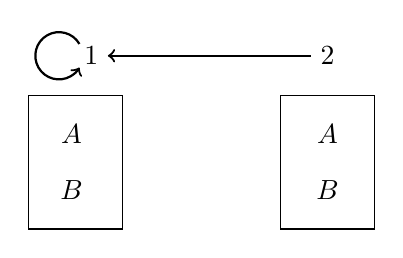
\begin{tikzpicture}
		\node (atom1) at (0,1) {1};
		\node (atom2) at (3,1) {2};
		\node (atom3) at (-0.25,0) {$A$};
		\node (atom4) at (3,0) {$\enot A$};
		\node (atom5) at (-0.25,-0.7) {$\enot B$};
		\node (atom6) at (3,-0.7) {$B$};
		\draw[->, thick] (atom1)+(-0.15,0.15) arc (-330:-30:.3);
		%\draw[->, thick] (atom2)+(0.15,-0.15) arc (-150:150:.3); 
		\draw[<-, thick] (atom1) -- (atom2);
		\draw (-0.8,-1.2) rectangle (0.4,0.5);
		\draw (2.4,-1.2) rectangle (3.6,0.5);
	\end{tikzpicture}
\end{center}
Qual a interpretação deste diagrama? Ele contém apenas dois mundos, 1 e 2. As setas entre os mundos indicam a relação de acessibilidade. Os mundos 1 e 2 acessam o mundo 1, mas nem 1 nem 2 acessam o mundo 2. As caixas em cada mundo nos permitem saber quais sentenças atômicas são verdadeiras em cada mundo: `$A$' é verdadeira em 1 mas  falsa em 2; `$B$' é falsa em 1 mas verdadeira em 2. Você só pode escrever uma sentença atômica ou a negação dela  em cada uma dessas caixas. A partir daí, podemos descobrir facilmente quais são os valores de verdade das sentenças complexas em cada mundo. Por exemplo, nessa interpretação, todas as sentenças a seguir são verdadeiras em $w_1$: 
 
\begin{itemize}
	\item[]$A\eand\enot B$, $B\eif A$, $\ediamond A$, $\ebox\enot B$
\end{itemize}
Se você não gosta de pensar diagramaticamente, também pode apresentar uma interpretação como esta:
\begin{itemize}
	\item[$W$:]$1,2$
	\item[$R$:]$\langle 1,1\rangle, \langle 2,1\rangle$
	\item[]$\nu_{1}(A)=V, \nu_{2}(B)=F, \nu_{2}(A)=F, \nu_{2}(B)=V$
\end{itemize}
Você terá a chance de preparar suas próprias interpretações 
em breve, quando começarmos a olhar para \emph{contrainterpretações}.

\section{Uma semântica para o Sistema \mlK}
\label{SemanticsK}

Agora podemos estender todos os conceitos semânticos da  LVF para cobrir também a LM:
\factoidbox{
	\begin{itemize}
		\item  $\metav{A}_1,\metav{A}_2, \dots \metav{A}_n\therefore\metav{C}$ é \xdefine{modalmente valido }se e somente se não há nenhum mundo em qualquer interpretação em que $\metav{A}_1,\metav{A}_2, \dots \metav{A}_n$ são todas verdadeiras e $\metav{C}$ é falsa.

		\item $\metav{A}$ é uma \xdefine{verdade modal} se e somente se $\metav{A}$ é verdadeira em todos os  mundos e   em todas as interpretações

		\item $\metav{A}$ é uma \xdefine{contradicao modal} se e somente se $\metav{A}$ é falsa em todos os mundos e em todas as interpretações.

		\item $\metav{A}$ is \xdefine{modalmente satisfatoria} se e somente se $\metav{A}$ é verdadeira  em algum mundo em alguma interpretação.
	\end{itemize}
}
(De agora em diante, deixaremos de lado as qualificações ``modais'' explícitas, uma vez que podem ser consideradas como lidas.)


Também podemos estender o uso de $\entails$. Para isso, precisamos adicionar subscritos da mesma forma como fizemos com $\proves$. Assim, quando quisermos dizer que $\metav{A}_1,\metav{A}_2, \dots \metav{A}_n\therefore\metav{C}$  é válido em \mlK, escreveremos: $\metav{A}_1,\metav{A}_2, \dots \metav{A}_n\entails_\mlK\metav{C}$. 

Para se ter uma ideia melhor desses conceitos semânticos, vejamos algumas contrainterpretações. Considere a seguinte afirmação (falsa):

\begin{itemize}
	\item[]
	      \begin{itemize}
		      \item[]$\enot A\entails_\mlK \enot \ediamond A$
	      \end{itemize}
\end{itemize}
Como obter uma contrainterpretação para essa afirmação? Precisamos construir uma interpretação na qual $\enot A$ é verdadeira em algum mundo $w$, e $\enot\ediamond A$ é falsa   nesse mundo $w$. Aqui está uma dessas interpretações, apresentada em um diagrama:
\begin{center}
	\begin{tikzpicture}
		\node (atom1) at (0,1) {1};
		\node (atom2) at (3,1) {2};
		\node (atom3) at (-0.25,0) {$\enot A$};
		\node (atom4) at (3,0) {$A$};
		\draw[->, thick] (atom1) -- (atom2);
		\draw (-0.8,-0.6) rectangle (0.4,0.5);
		\draw (2.4,-0.6) rectangle (3.6,0.5);
	\end{tikzpicture}
\end{center}
É fácil ver que isso funciona como uma contrainterpretação para  $\enot A\entails_\mlK\enot\ediamond A$. Em primeiro lugar, `$\enot A$' é verdadeira no mundo $1$. 
E, em segundo lugar, como `$A$' é verdadeira em $2$ e $2$ é acessível a partir de $1$, temos que `$\ediamond A$' é verdadeira em $1$, e consequentemente `$\enot\ediamond A$'   é falsa em $1$. 
Portanto, há algum mundo nessa interpretação onde `$\enot A$` é verdadeira e `$\enot\ediamond A$`  falsa.  

Por que escolhemos o subscrito \mlK? Existe uma relação importante entre o sistema \mlK{} e a definição de validade que acabamos de fornecer. Em particular, temos os dois resultados a seguir:
\begin{itemize}
	\item Se $\metav{A}_1,\metav{A}_2, \dots \metav{A}_n\proves_\mlK\metav{C}$, então $\metav{A}_1,\metav{A}_2, \dots \metav{A}_n\entails_\mlK\metav{C}$
	\item Se $\metav{A}_1,\metav{A}_2, \dots \metav{A}_n\entails_\mlK\metav{C}$, então $\metav{A}_1,\metav{A}_2, \dots \metav{A}_n\proves_\mlK\metav{C}$
\end{itemize}
O primeiro resultado é conhecido como \emph{correção}, pois nos diz que as regras de \mlK{} são boas e corretas: se você pode justificar um argumento fornecendo uma prova dele usando o sistema \mlK, então esse argumento é realmente válido. O segundo resultado é conhecido como    \emph{completude}, uma vez que nos diz que as regras de \mlK{} são amplas o suficiente para capturar todos os argumentos válidos: se um argumento é válido, então será possível oferecer uma prova em \mlK{} que o justifique.
 

Chamamos atenção para o fato de que uma coisa é anunciar esses resultados, outra bem diferente é prová-los. Não vamos provar esses resultados aqui, mas a ideia por trás da prova da correção talvez torne mais claro como funcionam as subprovas estritas.

Em uma subprova estrita, não  é permitido fazer uso de qualquer informação que esteja fora dela, exceto o que importamos para a subprova estrita usando  \ebox E. Se tivermos assumido ou provado $\ebox \metav{A}$, então por \ebox E  podemos usar $\metav{A}$ dentro de uma subprova estrita. E em \mlK, essa é a única maneira de importar uma fórmula para dentro de uma subprova estrita. Portanto, tudo o que pode ser provado dentro de uma subprova estrita deve seguir a partir de uma  fórmula  $\metav{A}$ onde fora da subprova estrita temos $\ebox \metav{A}$. Vamos imaginar que estejamos raciocinando sobre o que é verdade em um mundo possível em alguma interpretação. Se sabemos que $\ebox\metav{A}$ é verdadeira em um mundo possível, então sabemos que $\metav{A}$ é verdadeira em todos os mundos acessíveis a ele. Portanto, tudo o que for provado dentro de uma subprova estrita é verdadeiro em todos os mundos possíveis acessíveis a esse mundo. É por isso que \ebox I é uma regra correta.

\section{Uma semântica para o sistema \mlT}
\label{SemanticsT}

Dissemos que o sistema \mlK{} é correto e completo em relação à definição de validade que demos acima. Mas,  o que podemos afirmar sobre os outros sistemas modais \mlT, \mlSfour{}  e \mlSfive  ? Bem, eles são todos  \emph{incorretos} com respeito a essa definição de validade. Por exemplo, todos esses sistemas permitem inferir $A$ a partir de $\ebox A$, embora  $\ebox A\nentails_\mlK A$.

Isso significa que esses sistemas são uma perda de tempo? De jeito nenhum! Esses sistemas são apenas incorretos \emph{em relação à definição de validade que demos acima}. (Ou, usando símbolos, eles não são corretos em relação a $\entails_\mlK$.) Assim, quando estamos lidando com esses sistemas modais mais fortes, precisamos apenas modificar nossa definição de validade. É aqui que as relações de acessibilidade são realmente úteis.

Quando introduzimos a ideia de uma relação de acessibilidade, dissemos que poderia ser qualquer relação entre mundos de que você goste: você poderia tê-la relacionando todos os mundos a todos os mundos,  nenhum mundo para nenhum mundo, ou qualquer coisa no meio. É assim que pensamos as relações de acessibilidade em nossa definição de $\entails_\mlK$. Mas se quiséssemos, poderíamos  colocar algumas restrições na relação de acessibilidade. Em particular, podemos impor que a relação de acessibilidade seja \emph{reflexiva}:

\begin{itemize}
	\item $\forall wRww$
\end{itemize}
Isto significa que todo mundo acessa ele próprio. Ou em termos de possibilidade relativa: todo mundo é possível em relação a si mesmo. Com   essa restrição podemos introduzir uma nova relação de consequência, $\entails_\mlT$, como segue:
\factoidbox{
	$\metav{A}_1,\metav{A}_2, \dots \metav{A}_n\entails_\mlT \metav{C}$  se e somente se  não existe nenhum mundo em qualquer interpretação \emph{que tenha uma relação de acessibilidade reflexiva}, na qual $\metav{A}_1,\metav{A}_2, \dots \metav{A}_n$ são todas verdadeiras e $\metav{C}$ é falsa.
}
Anexamos o subscrito \mlT{}  a $\entails$ porque verifica-se que o sistema \mlT{} é correto e completo em relação a esta nova definição de validade:
\begin{itemize}
	\item Se $\metav{A}_1,\metav{A}_2, \dots \metav{A}_n\proves_\mlT\metav{C}$, então $\metav{A}_1,\metav{A}_2, \dots \metav{A}_n\entails_\mlT\metav{C}$
	\item Se $\metav{A}_1,\metav{A}_2, \dots \metav{A}_n\entails_\mlT\metav{C}$, então $\metav{A}_1,\metav{A}_2, \dots \metav{A}_n\proves_\mlT\metav{C}$
\end{itemize}
Como antes, não provaremos os resultados de correção e completude. No entanto, é relativamente fácil  justificar a regra  R\mlT, se a relação de acessibilidade for 
reflexiva.

\factoidbox{
	\[\begin{nd}
			\have[m]{m}{\ebox \metav{A}}
			\have[\, ]{n}{\metav{A}}\rt{m}
		\end{nd}\]
}
Para mostrar isto é suficiente mostrar que não existe uma  contrainterpretação para:
\[
	\ebox \metav{A}\entails_\mlT \metav{A}
\]
 
Caso existisse,  precisaríamos construir  uma interpretação  na qual $\ebox \metav{A}$ fosse verdadeira em algum  mundo  $w$, mas $\metav{A}$ fosse falsa nesse mundo. Agora, se $\ebox \metav{A}$ é verdadeira em $w$, então $\metav{A}$ deve ser verdadeira em todos os mundos acessíveis a $w$. Mas como a relação de acessibilidade é reflexiva, $w$ acessa $w$. Logo, $\metav{A}$ deve ser verdadeira também em $w$. 
Chegamos assim a uma contradição,  pois assumimos que
  $\metav{A}$ era falsa em $w$. 

\section{Uma semântica para \mlSfour}
\label{SemanticsS4}

De que outra forma podemos ajustar nossa definição de validade? Podemos também estipular que a relação de acessibilidade seja \emph{transitiva}:
\begin{itemize}
	\item $\forall w_1\forall w_2\forall w_3 ((Rw_1w_2 \eand Rw_2w_3)\eif Rw_1w_3)$
\end{itemize}
Isso significa que se  $w_1$ acessa $w_2$, e $w_2$ acessa $w_3$, então  $w_1$ acessa $w_3$. Ou em termos de possibilidade relativa: se $w_3$ é possível em relação a $w_2$, e $w_2$ é possível em relação a  $w_1$, então $w_3$ é possível em relação a  $w_1$. Com essa restrição imposta  à nossa relação de acessibilidade, temos uma nova relação de consequência, $\entails_\mlSfour$, como segue:
\factoidbox{
	$\metav{A}_1,\metav{A}_2, \dots \metav{A}_n\entails_\mlSfour \metav{C}$ se e somente se não existe nenhum mundo em qualquer interpretação \emph{que tenha uma relação de acessibilidade reflexiva e transitiva}, na qual $\metav{A}_1,\metav{A}_2, \dots \metav{A}_n$ são todas verdadeiras e $\metav{C}$ é falsa
}
Anexamos o subscrito \mlSfour{}  a $\entails$ porque verifica-se que o sistema \mlSfour{} é correto e completo em relação a esta nova definição de validade:
\begin{itemize}
	\item Se $\metav{A}_1,\metav{A}_2, \dots \metav{A}_n\proves_\mlSfour\metav{C}$, então $\metav{A}_1,\metav{A}_2, \dots \metav{A}_n\entails_\mlSfour\metav{C}$
	\item Se $\metav{A}_1,\metav{A}_2, \dots \metav{A}_n\entails_\mlSfour\metav{C}$, então $\metav{A}_1,\metav{A}_2, \dots \metav{A}_n\proves_\mlSfour\metav{C}$
\end{itemize}
Como antes,  não  provaremos os resultados de correção e completude.  No entanto, é relativamente fácil  justificar a regra   R$\mathbf{4}$,  se a relação de acessibilidade for transitiva.
 
\factoidbox{
	\[\begin{nd}
			\have[m]{m}{\ebox\metav{A}}
			\open
			\hypo[\ ]{k}{\ebox}
			\have[\ ]{n}{\ebox\metav{A}}\rfour{m}
		\end{nd}\]
}
Lembramos que a ideia por trás das subprovas estritas é que elas são maneiras de provar coisas que devem ser verdadeiras em todos os mundos acessíveis. Assim, a regra R$\mathbf{4}$  significa que sempre que $\ebox \metav{A}$ for verdadeira em um mundo, $\ebox \metav{A}$ também deve ser verdadeira  em todos os mundos acessíveis  a este mundo. Logo, devemos ter $\ebox\metav{A} \entails_\mlSfour \ebox\ebox\metav{A}$.

Para constatar isso, tente construir uma contrainterpretação para esta afirmação:
\begin{itemize}
	\item[]$\ebox\metav{A} \entails_\mlSfour \ebox \ebox \metav{A}$
\end{itemize}
Precisaríamos construir uma interpretação na qual $\ebox\metav{A}$ seja verdadeira em um mundo  $w_1$, mas  $\ebox \ebox \metav{A}$  falsa nesse mundo. Agora, se $\ebox \ebox \metav{A}$  é falsa em  $w_1$, então  $w_1$ deve acessar algum mundo, $w_2$, no qual $\ebox\metav{A}$ é falsa. Da mesma forma, se $\ebox \metav{A}$ é falsa em $w_2$, então $w_2$ deve acessar algum mundo, $w_3$, no qual $\metav{A}$ é falsa. Acabamos de dizer que  $w_1$ acessa $w_2$, e $w_2$ acessa $w_3$. Logo,  $w_1$ acessa $w_3$, pois a relação de acessibilidade é  transitiva.  Por outro lado, do fato de $\ebox\metav{A}$  ser verdadeira em $w_1$, segue que   $\metav{A}$  é verdadeira em todo mudo acessível a $w_1$, em particular, verdadeira em $w_3$.  Portanto, $\metav{A}$ é verdadeira e falsa em $w_3$. Contradição!

\section{Uma semântica para  \mlSfive}
\label{SemanticsS5}

Vamos acrescentar mais uma restrição à relação de acessibilidade. Desta vez, impor que a relação de acessibilidade seja também \emph{simétrica}:
\begin{itemize}
	\item $\forall w_1\forall w_2(Rw_1w_2 \eif Rw_2w_1)$
\end{itemize}
Isto significa que se  $w_1$ acessa $w_2$, então $w_2$ acessa  $w_1$. Ou em termos de possibilidade relativa: se $w_2$ é possível em relação a  $w_1$, então  $w_1$ é possível em relação a $w_2$. Os lógicos chamam uma relação que é reflexiva, simétrica e transitiva de \emph{relação de equivalência}. Agora podemos  definir uma nova relação de consequência, $\entails_\mlSfive $, como segue:

\factoidbox{
	$\metav{A}_1,\metav{A}_2, \dots \metav{A}_n\entails_\mlSfive  \metav{C}$ se e somente se  não existe nenhum mundo em qualquer interpretação \emph{cuja relação de acessibilidade seja uma relação de equivalência}, na qual $\metav{A}_1,\metav{A}_2, \dots \metav{A}_n$ são todas verdadeiras e $\metav{C}$ é falsa.
}
Anexamos o subscrito \mlSfive{} a $\entails$ porque  o sistema \mlSfive{} é correto e completo em relação a esta nova definição de validade:

\begin{itemize}
	\item Se $\metav{A}_1,\metav{A}_2, \dots \metav{A}_n\proves_\mlSfive \metav{C}$, então $\metav{A}_1,\metav{A}_2, \dots \metav{A}_n\entails_\mlSfive \metav{C}$
	\item Se $\metav{A}_1,\metav{A}_2, \dots \metav{A}_n\entails_\mlSfive \metav{C}$, então $\metav{A}_1,\metav{A}_2, \dots \metav{A}_n\proves_\mlSfive \metav{C}$
\end{itemize}
Como antes,  não  provaremos os resultados de correção e completude.  No entanto, é relativamente fácil  justificar  a regra R$\mathbf{5}$,  se a relação de acessibilidade for uma relação de equivalência.

\factoidbox{
	\[\begin{nd}
			\have[m]{m}{\enot\ebox \metav{A}}
			\open
			\hypo[\ ]{k}{\ebox}
			\have[\, ]{n}{\enot\ebox\metav{A}}\rfive{m}
		\end{nd}\]
}
Essa regra diz que se $\metav{A}$ não é necessária, ou seja, falsa em algum mundo acessível, também não é necessária em qualquer mundo possível acessível. Temos então $\enot\ebox \metav{A} \entails_\mlSfive  \ebox\enot\ebox \metav{A}$.

Para constatar isso, tente construir uma contrainterpretação para esta afirmação:
\[
	\enot\ebox\metav{A} \entails_\mlSfive  \ebox \enot\ebox \metav{A}
\]
 
Precisaríamos construir uma interpretação  na qual  $\enot\ebox\metav{A}$ é verdadeira em um mundo $w_1$, mas  $\ebox \enot\ebox \metav{A}$  é falsa nesse mundo.  Agora, se $\enot\ebox\metav{A}$ é verdadeira em  $w_1$, então  $w_1$ deve acessar algum mundo, $w_2$, no qual $\metav{A}$ é falsa. Da mesma forma, se $\ebox \enot\ebox \metav{A}$ é falsa em  $w_1$, então  $w_1$ deve acessar algum mundo, $w_3$, no qual $\enot\ebox \metav{A}$ é falsa. Como agora temos a restrição que a relação de acessibilidade é uma relação de equivalência e, portanto, simétrica, podemos inferir que $w_3$ acessa  $w_1$. Assim, $w_3$ acessa  $w_1$, e  $w_1$ acessa $w_2$. Novamente, como a relação de acessibilidade é uma relação de equivalência e, portanto, transitiva, podemos inferir que $w_3$ acessa $w_2$. Mas antes dissemos que $\enot\ebox \metav{A}$ é falsa em $w_3$, o que implica que $\metav{A}$ é verdadeira em todos os mundos que $w_3$ acessa. Portanto, $\metav{A}$ é verdadeira e falsa em $w_2$. Contradição!

Na definição de  $\entails_\mlSfive $, estipulamos que a relação de acessibilidade deve ser uma relação de equivalência. Mas acontece que há outra maneira de obter uma noção de validade adequada para \mlSfive. Em vez de estipular que a relação de acessibilidade seja uma relação de equivalência, podemos estipular que seja uma relação \emph{universal}:
\begin{itemize}
	\item $\forall w_1\forall w_2Rw_1w_2$
\end{itemize}
Isto significa  que todo mundo acessa todo mundo. Ou em termos de possibilidade relativa: todo mundo é possível em relação a todo mundo. Usando essa restrição na relação de acessibilidade, poderíamos ter definido  $\entails_\mlSfive $ assim:\factoidbox{
	$\metav{A}_1,\metav{A}_2, \dots \metav{A}_n\entails_\mlSfive  \metav{C}$ se e somente se  não existe nenhum mundo em qualquer interpretação  \emph{que tenha uma relação de acessibilidade universal}, na qual $\metav{A}_1,\metav{A}_2, \dots \metav{A}_n$ são todas verdadeiras e $\metav{C}$ é falsa.
}
Se definíssemos $\entails_\mlSfive $ assim, ainda obteríamos os mesmos resultados de correção e completude para \mlSfive{}. O que isso nos diz? Isso significa que se estamos lidando com uma noção de necessidade segundo a qual todo mundo é possível em relação a todo mundo, então devemos usar \mlSfive{}. Além disso, a maioria dos filósofos assume que as noções de necessidade com as quais estão mais preocupados, como a necessidade lógica e a \emph{necessidade metafísica}, são exatamente desse tipo. Portanto, \mlSfive{} é o sistema modal que a maioria dos filósofos usa na maior parte do tempo.
 

\practiceproblems

\problempart
Apresente contrainterpretações para as quatro seguintes afirmações falsas:
\begin{earg}
	\item $\enot P \entails_\mlK \enot\ediamond P$
	\item $\ebox(P \eor Q)\entails_\mlK \ebox P \eor \ebox Q$
	\item $\entails_\mlK \enot \ebox (A\eand \enot A)$
	\item $\ebox A\entails_\mlK A$
\end{earg}

\problempart
Apresente contrainterpretações para as duas seguintes afirmações falsas:
\begin{earg}
	\item $\ebox (M\eif O),\ediamond M\entails_\mlT O$
	\item $\ebox A\entails_\mlT \ebox \ebox A$
\end{earg}

\problempart
Apresente contrainterpretações para as duas seguintes afirmações falsas:
\begin{earg}
	\item $\ediamond A\entails_\mlSfour \ebox\ediamond A$
	\item $\ediamond A, \ebox (\ediamond A \eif B)\entails_\mlSfour\ebox B$
\end{earg}

\section*{Leitura adicional}

A lógica modal é um grande subcampo da lógica. Nós apenas arranhamos a superfície. Se você quiser aprender mais sobre lógica modal, aqui estão alguns livros que você pode consultar:

\begin{itemize}
	\item Hughes, G. E., \& Cresswell, M. J. (1996). \emph{A New Introduction to Modal Logic}, Oxford: Routledge.
	\item Priest, G. (2008). \emph{An Introduction to Non-Classical Logic}, 2nd ed., Cambridge: Cambridge University Press.
	\item Garson, J. W. (2013). \emph{Modal Logic for Philosophers}, 2nd ed., Cambridge: Cambridge University Press.
\end{itemize}

Nenhum desses autores formula seus sistemas de provas modais da mesma forma que nós, mas a formulação mais próxima é dada por Garson. 



